\begin{figure}[H]
\centering
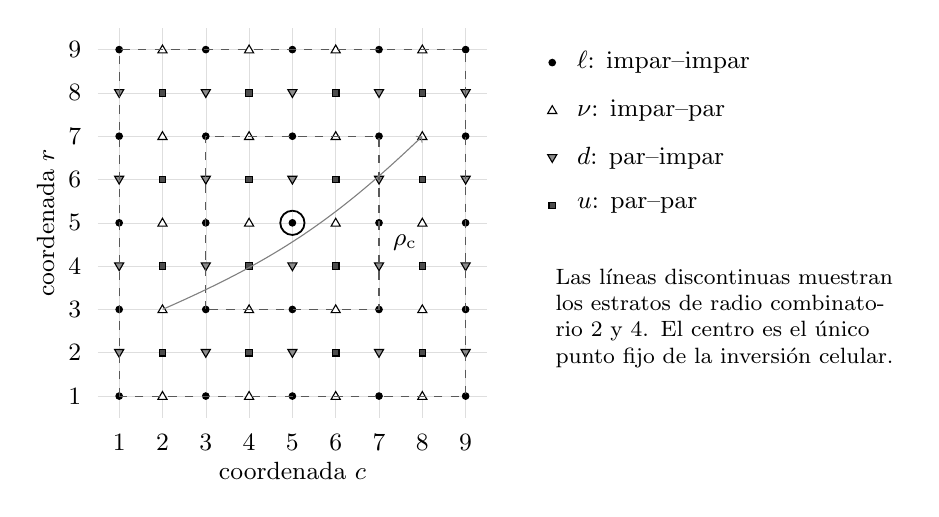
\begin{tikzpicture}[x=.55cm,y=.55cm, every node/.style={font=\small}]
  \draw[step=1,black!13,very thin] (.5,.5) grid (9.5,9.5);
  \foreach \k in {1,...,9} {
    \node[below] at (\k,.35) {$\k$};
    \node[left] at (.35,\k) {$\k$};
  }
  \node[below] at (5,-.3) {coordenada $c$};
  \node[rotate=90] at (-.7,5) {coordenada $r$};
  \foreach \r in {1,...,9} {
    \foreach \c in {1,...,9} {
      \pgfmathtruncatemacro{\pr}{mod(\r,2)}
      \pgfmathtruncatemacro{\pc}{mod(\c,2)}
      \ifnum\pr=1
        \ifnum\pc=1
          \draw[fill=black] (\c,\r) circle (.075);
        \else
          \draw[fill=white] (\c,\r+.105)--(\c-.105,\r-.075)--(\c+.105,\r-.075)--cycle;
        \fi
      \else
        \ifnum\pc=1
          \draw[fill=black!45] (\c,\r-.105)--(\c-.105,\r+.075)--(\c+.105,\r+.075)--cycle;
        \else
          \draw[fill=black!70] (\c-.075,\r-.075) rectangle (\c+.075,\r+.075);
        \fi
      \fi
    }
  }
  \draw[black!65,dashed] (3,3) rectangle (7,7);
  \draw[black!65,dashed] (1,1) rectangle (9,9);
  \draw[line width=.65pt] (5,5) circle (.28);
  \draw[->,black!50] (2,3) to[bend right=10] (8,7);
  \node[fill=white,inner sep=2pt] at (7.6,4.55) {$\rho_{\mathrm c}$};
  \begin{scope}[shift={(11,8.7)}]
    \draw[fill=black] (0,0) circle (.075);
    \node[right] at (.35,0) {$\ell$: impar--impar};
    \draw[fill=white] (0,-.995)--(-.105,-1.175)--(.105,-1.175)--cycle;
    \node[right] at (.35,-1.1) {$\nu$: impar--par};
    \draw[fill=black!45] (0,-2.305)--(-.105,-2.125)--(.105,-2.125)--cycle;
    \node[right] at (.35,-2.2) {$d$: par--impar};
    \draw[fill=black!70] (-.075,-3.375) rectangle (.075,-3.225);
    \node[right] at (.35,-3.3) {$u$: par--par};
    \node[anchor=west,text width=4.4cm,align=left,font=\footnotesize]
      at (-.15,-5.9) {Las líneas discontinuas muestran los estratos de radio combinatorio $2$ y $4$. El centro es el único punto fijo de la inversión celular.};
  \end{scope}
\end{tikzpicture}
\caption[Clasificación sobre el atlas posicional]{Clasificación sobre el atlas posicional. Las marcas distinguen las
cuatro clases internas de paridad, anteriores a sus realizaciones físicas.
La profundidad se mide con $g(r,c)=\max(|r-5|,|c-5|)$.
La flecha ilustra $(2,3)\mapsto(8,7)$ bajo la inversión celular;
no representa una trayectoria dinámica ni un cambio de sabor.
El círculo central marca $(5,5)$, de profundidad cero.}
\label{vi:fig:atlas}
\end{figure}
